\chapter{Characteristics of a sensor}
When designing a mechatronic system, sensor is crucial for data acquisition and generating an adequate response. However, if a engineer only relies on the best available sensor, the product price will be higher than necessary, resulting in customers lost to competitive manufacturers. Therefore, this chapter is dedicated to accommodate selecting the right sensor for one's application with common characteristics available on datasheets.

\section{Mobile Communication Devices}
\begin{figure}[ht]
	\centering
	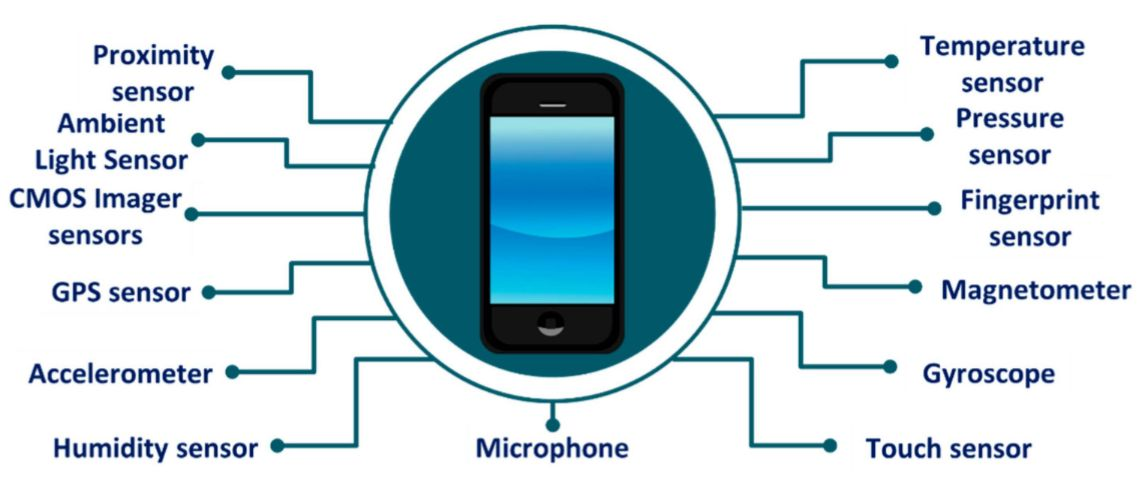
\includegraphics{mcd}
	\caption{Built-in sensors in a typical present-day smartphone}
\end{figure}
Mobile Communication Devices (MCD) sensors are designed for portability and full integration with other components inside a hand-held device. It is a self-containing sensing module that detects, conditions, digitizes, processes, outputs and communicates information while being small, light, accurate, stable, fast-response, etc. A generic purpose device (e.g. smartphones, tablets, smartwatches) contains dozens of them for different applications and is categorized in 4 areas:
\begin{enumerate}
	\item \textbf{Industrial} for detecting noncontact tempertaure, thermal imaging, humidity, air flow ionizing radiation, smell, diaelectric constant of objects, maerial composition, range (distance), air pressure, produce freshness, etc.
	\item \textbf{Medical} for the inner (core) and skin body temperatures, thermal imaging, arterial blood pressure, EKG, blood factors (glucose, cholesterol, hemoglobin oxygen saturation), deep body imaging, smell (e-nose), behavior modification, etc.
	\item \textbf{Military} for night vision, detecting poisonous gases, proximity, ionizing radiation, explosives, chemical and biological agents, etc.
	\item \textbf{Consumer} for the body core temperature, heart rate, radon gas, pregnancy detection, breathalizer for alcohol and hydrogen sulfide, food composition, behavior modification, proximity, V level, electromagnetic pollution, surface temperature, etc.
\end{enumerate}

\section{Full-Scale Input/Output}
A \textit{span} or an \textit{input full scale} (FS) is a dynamic range of stimuli convertible by a sensor. In a datasheet, it is regarded as the highest possible input value without causing unacceptably large error. For sensors with broad response characteristics, the span is often expressed in decibels, which is a logarithmic measure of ratios of either power or force (voltage).

A \textit{full-scale output} (FSO) for an analog output is the difference between electrical output signals at 2 ends of the input signals. For digital output, it is the maximum digital count the A/D converter can resolve for maximum FS.

\section{Accuracy}
It is defined as \textit{maximum}, or \textit{typical}, or \textit{average} error of the sensor alone. The rating of accuracy is represented in 4 common forms, depending on the application:
\begin{enumerate}
	\item \textit{Directly in terms of measured value of a stimulus}, which is used when error is independent on the input signal magnitude.
	\item \textit{In percentage of FS}, which is useful for a sensor with a linear transfer function and can be thought as an alternative of the approach above. For nonlinear transfer function, the representation may be misleading.
	\item \textit{In percentage of the measured signal}, which is useful for a nonlinear transfer function, even with very dynamic inputs. However, the error typically does not proportionally scale with the input magnitude.
	\item \textit{In terms of the output signal}, which is useful for sensors with a digital output format.
\end{enumerate}
In reality, a datasheet mixes 2 or more forms and take whichever value is the largest. In this way, the error can be evaluated more accurately.

\section{Possible types of error}
In a datasheet, tolerance and error limit are paramount for any measuring equipment, which the manufacture always dedicates a section for. Distinguishing the types of error is helpful to determine the suitable sensor for designing a mechatronic system. Generally, there are 6 types of error:
\paragraph{Calibration error}
Calibration error occurs while adjusting a sensor. In dynamic system and control, it is categorized as \textit{disturbance}, which is quantitative data and contributes the systematic error. Another source of errors regarding calibration is a reference sensor. This type of sensor is considered as national standard, which all manufactured sensors rely on. Therefore, for absolute accuracy, the error from "standardized sensors" is considered.
\paragraph{Hysteresis error}
Hysteresis error is the maximum deviation between output values given the same input signal. For example, if the sensitivity of the sensor is $ 10\unit{mV/mm} $, the hysteresis error in terms of displacement units is $ 2\unit{mm} $. Possible causes of this faulty result are geometry of design, friction or deformation of material.
\paragraph{Nonlinearity error}
If the error is assumed to , nonlinearity error will be specified to compensate for any faulty assumptions. It is the maximum deviation of a real transfer function from the approximation straight line. After several calibration runs, the worst linearity result is stated. This type of error is crucial if the output signal requires best accuracy in a small range (e.g. medical thermometer measures body temperature between $ 36-38^\circ\text{C} $). Oftentimes, manufacturers are inclined to publish the smallest possible nonlinearity error without specifying what approximation method is used.
\begin{figure}
	\centering
	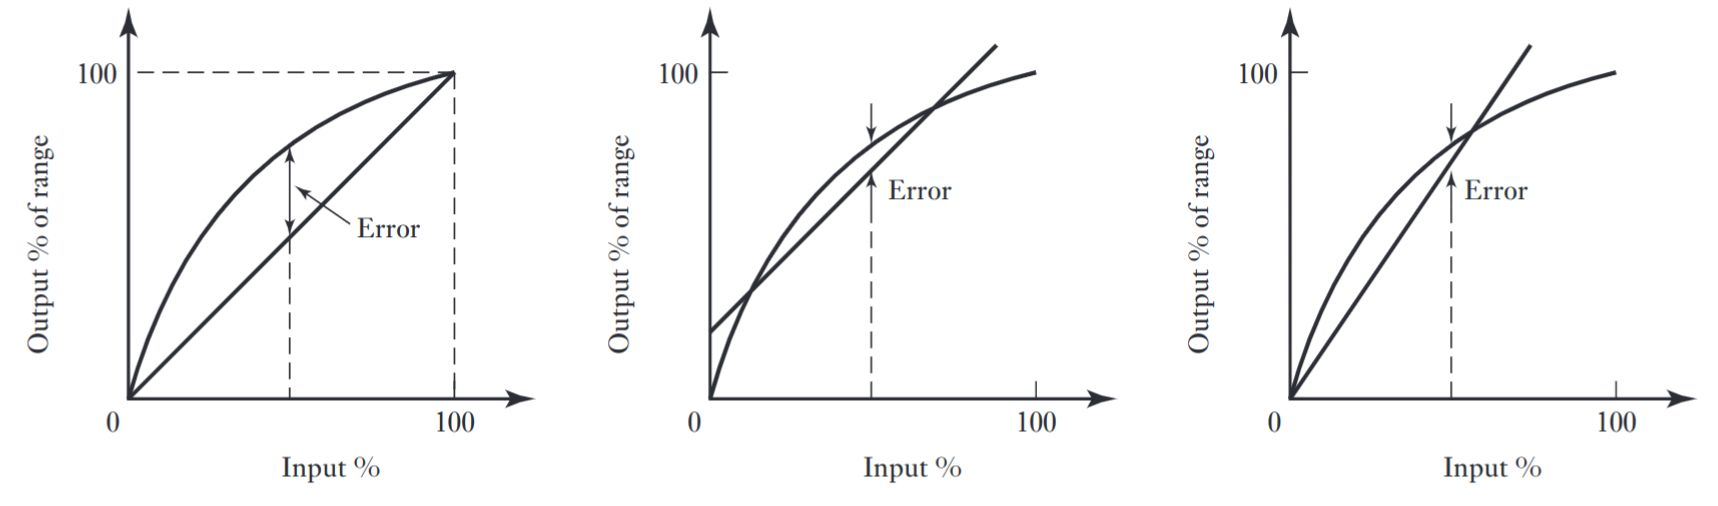
\includegraphics[width=\linewidth]{hysteresis}
	\caption{Non-linearity error using (from left to right): end-range values; best straight line for all values; best straight line through the zero point \cite{bolton2015mechatronics}}
\end{figure}
\paragraph{Saturation error}
Saturation error occurs when the input signal exceeds the operating limit of a sensor.
\paragraph{Repeatability error}
Repeatability error causes a sensor to output different values under identical conditions. Possible noises for the error are thermal conductivity, charge, deformation, etc.
\paragraph{Dead band error}
Dead band error is the insensitivity of a sensor in a specific range of the input signals, which generates output signals between a certain value (often zero).
\section{Resolution}
Digital input-output signals are not continuous as shown in the figures in a datasheet but rather distinguish data points. The distance between 2 consecutive data points is defined as resolution. Depending on manufacturers, the step size may be specified as typical, average, or worst.
\section{Special output characteristics}
Depending on sensor types, specifying input properties might be necessary. For instance, in case of flow sensors, thermal transport sensors require identifying temperature bandwidth to give the accurate response.
\paragraph{Impedance}
When working with an electronic sensor, the output impedance of the sensor $ Z_{out} $ and the input impedance of the connecting system $ Z_{in} $ should be acknowledge. A current generating sensor should have high $ Z_{out} $ and low $ Z_{in} $. This is the opposite for voltage generating sensor.
\paragraph{Format}
For mechatronic systems, programming a microcontroller or microprocessor needs the output format of the sensor. The output electrical characteristics may include voltage, current, charge, frequency, amplitude, phase, polarity, shape of a signal, time delay and digital code. These responses can be displayed in formats such as binary, text (ASCII), or digital output, etc. with various forms of communication (e.g. serial link, PWM, $ I^2C $).
\paragraph{Excitation}
Analogues to a match catching fire with a spark, excitation signal could be included in a datasheet. An exapmle of an excitation signal is electric current passing through a thermistor to measure its temperature-dependent resistance.
\paragraph{Dynamic characteristics}
Besides from steady input signals, dynamic and time-varying stimuli are also considered. The sensor responses slowly to this input type, which generates dynamic error. At best, the error is a delay. At worst, it causes undesirable oscillations. In such cases, Dynamic Systems and Control course is provided to discuss extensively about this topic.
\section{Environmental factors}
Generally, all possible environmental factors that may affect the sensor performance are specified by manufacturers. In a datasheet, it is typical to include information about the following factors:
\begin{enumerate}
	\item \textit{Storage condition}, which specifies the highest and lowest storage temperature. It also has maximum relative humidities at these temperatures and may be mentioned as "noncondensing". Along with operating temperature range, this information is \textit{one of the most common environmental factors} available in any datasheet. 
	\item \textit{Short-term stability} is manifested as changes in the sensor's performance within minutes, hours, or days, which essentially is another way to express bidirectional repeatability.
	\item \textit{Long-term stability} is the irreversible change in the material's electrical, mechanical, chemical or thermal properties. Similar to heat treated materials, a sensor can improve its stability by \textit{pre-aging}. For instance, a sensor may be periodically swung from freezing to hot temperatures before being calibrated and installed into a product.
	\item \textit{Environmental conditions during normal operation} affects the transfer function of a sensor. An example is a strain gauge whose sensitivity increases with temperature. Even if the manufacture does not specify these conditions in the datasheet, it is the responsibility of an engineer to simulate and prototype the end-product corresponding to the environment.
\end{enumerate}
\section{Reliability}
In statistical terms, reliability is the probability that the device will function without failure over a specified time or a number of uses. Reliability specifies a failure  is a temporary or permanent malfunction of a device. Although this is an important property of a sensor, the information is not readily available in most datasheet due to the absence of measuring standards of reliability. Therefore, an engineer should be ready to do the test by any means. Some example testing procedures are MTBF, extreme testing, accelerated life testing, HALT testing, FOAT testing, etc.
\section{Application characteristics}
This information includes geometry and other simple physical specifications such as design, weight, power consumption and overall dimensions. Although price heavily influences a sensor's performance, any amount of cost is justified if reliability and accuracy are of a paramount importance.
\section{Uncertainty}
While error is what we unknowably get when we measure, uncertainty is what we think how large that error might be. No matter how well a sensor is made, there always exists obscure factors. Even if they are recognized, it is impossible to measure exactly (e.g. human factor). Attempts have been made to quantitatively identify them: evaluation through statistical methods, preceding measurement data, personal experience, manufacturer's specifications, uncertainty data referenced from handbooks and manuals, etc.
